\section{Overall System Design}

The PARSE toolkit is being designed as a standalone application to run in the Windows environment. The novel nature of the functionality that is being implemented and the cross compatible nature of the Kinect API with several high level languages meant that there was little software available that could be extended or re-developed. The modular nature of the design and the plug and play nature of the Kinect lends the toolkit to further development through open source means.\\

The system's functionality is pipelined, which each functionality consisting of a chain of processing elements. Each processing element is a \emph{filter} connected by \emph{pipes} which are then eventually fed back to to the central module of the system which dispatches commands to these pipelines. This analogy and method of architecting the system is appropriate given the stream-like nature of the raw data that is received by the Kinect sensor. \\

\begin{center}
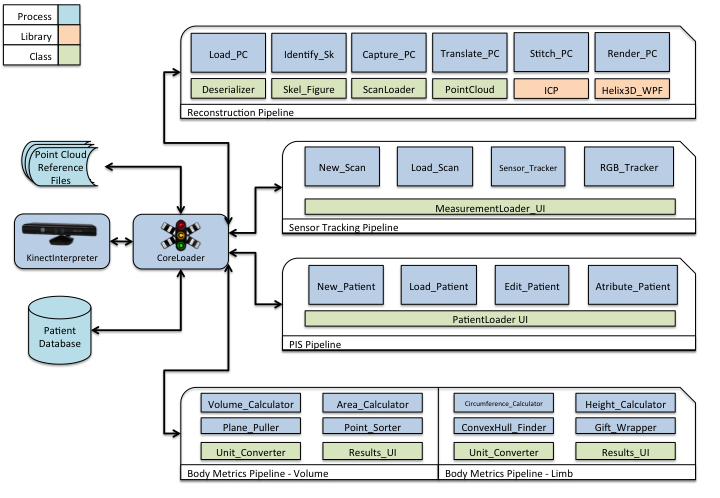
\includegraphics[scale=0.7, angle=90]{images/Slide1.png}
\caption{High-level system design with key classes and libraries highlighted}
\end{center}

\subsection{Workflow Description}
The system consists of 4 key functionalities, the scanning of a patient, the calculation of whole body volume or limb circumference, the tracking and recall of a sensor's position relative to the body and the management of patient information. Each of these functionalities is predicated on having access to a Kinect device or access to previous scans. Each of these functions can be accessed via a central class which handles the interfacing requirements of the Kinect through a dedicated interpreter class as well as performing message passing between the various subclasses and the Kinect device. \\

Each function consists of a specific use case. These are outlined below and in most cases consist of a single actor, the doctor, carrying out operations which indirectly involve the patient through means of scan capture or scan recognition. \\

\emph{\bf{Scan Capture and Retrieval}}\\

The diagram below describes the operations involved in capturing a scan and then it's subsequent retrieval.\\

\begin{figure}[!h]
\begin{center}
    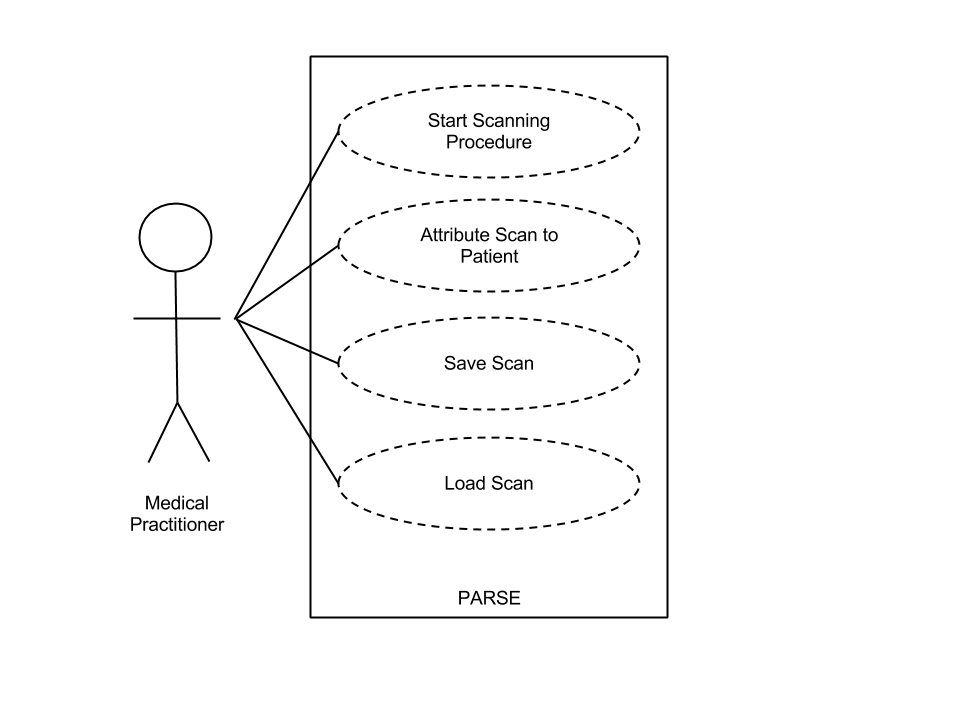
\includegraphics[scale=0.25]{images/uml1.png}
\end{center}
\end{figure}

\pagebreak

\emph{\bf{Volume Reconstruction}}\\

The diagram below shows the operations that can be applied when the scan has been completed and that volume reconstruction is ready to be applied or recalled.\\

\begin{center}
    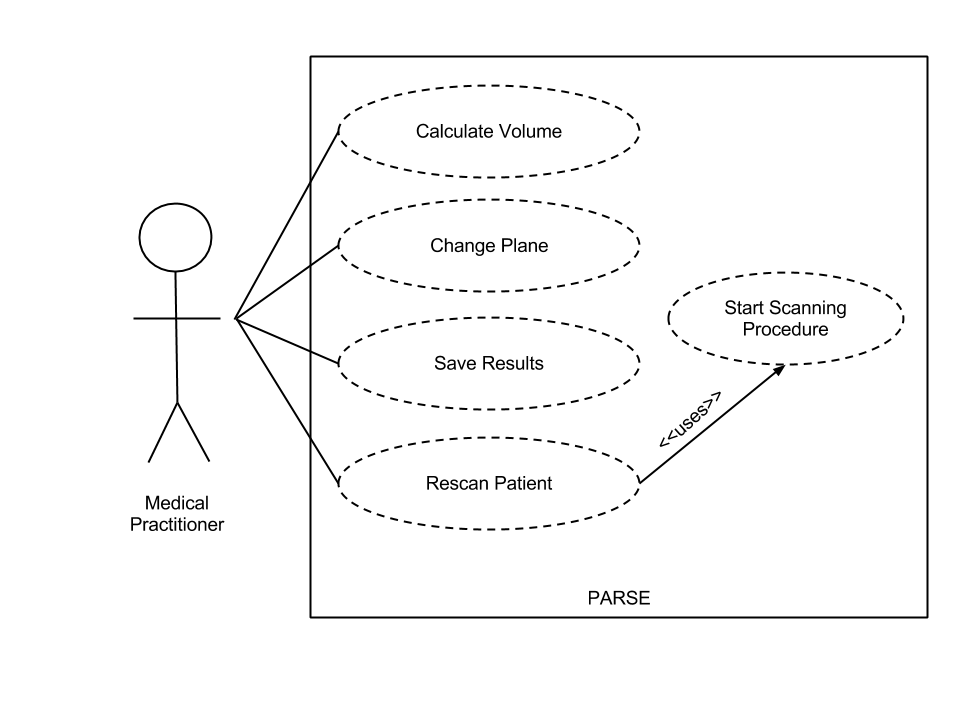
\includegraphics[scale=0.275]{images/uml2.png}
\end{center}

\emph{\bf{Limb Circumference}}\\

This diagram outlines the operations involved in calculating limb circumference. \\

\begin{center}
    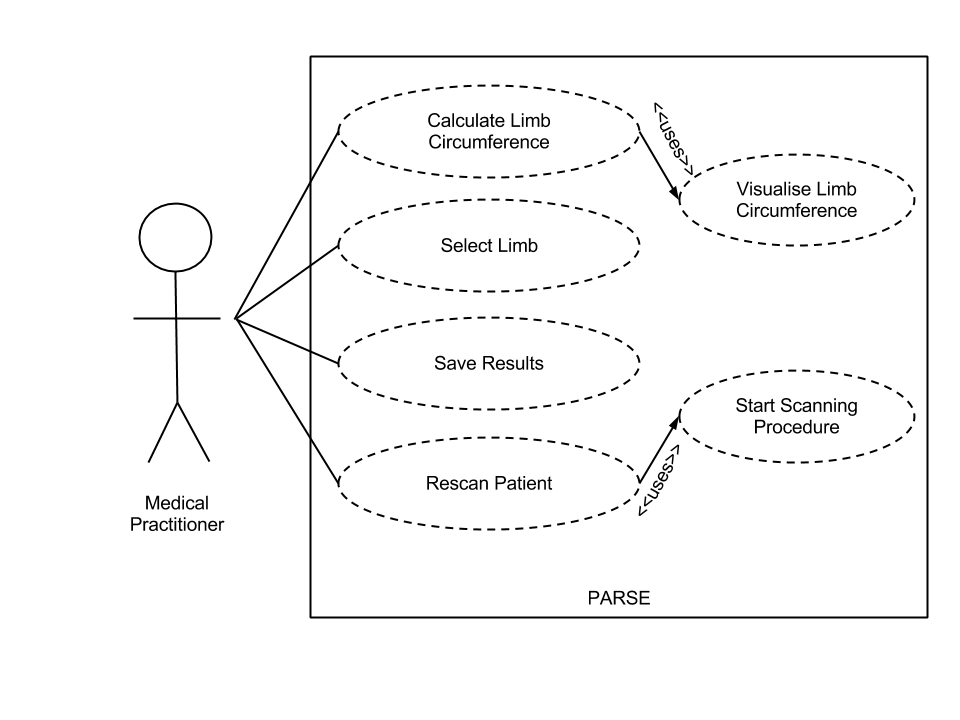
\includegraphics[scale=0.275]{images/uml3.png}
\end{center}

\emph{\bf{Markerless Recording and Reconstruction}}\\

This diagram shows what is involved in the process of recording a markerless scan and then reconstructing the results when the scan needs to be recalled. \\

\begin{center}
    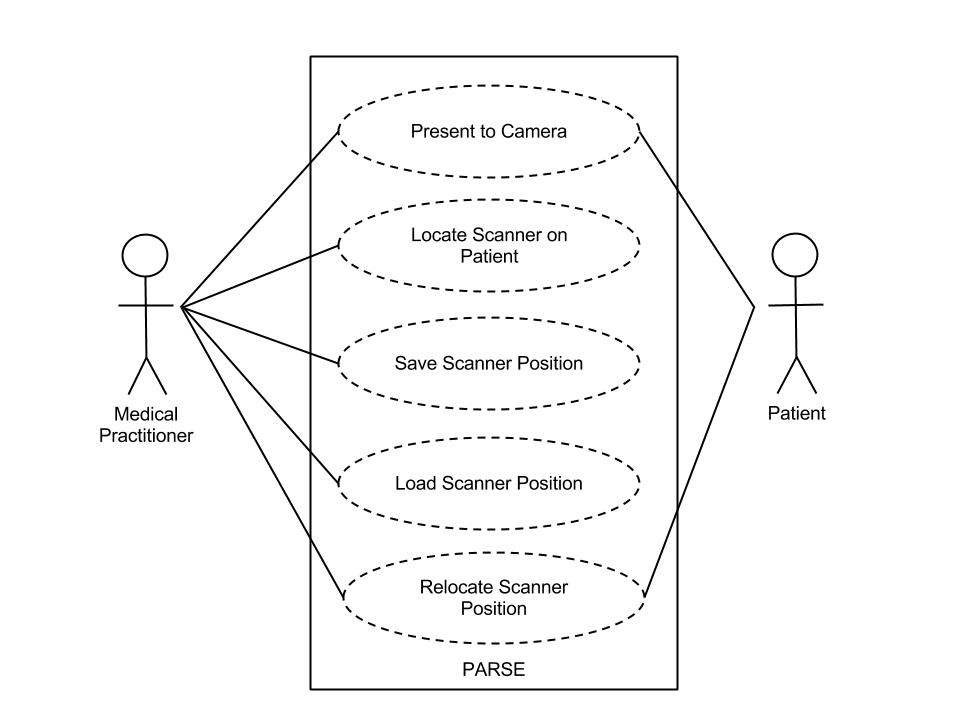
\includegraphics[scale=0.275]{images/uml4.png}
\end{center}

\pagebreak

\emph{\bf{Patient Information Management}}\\

This diagram shows the operations involved in managing patient information. \\

\begin{center}
    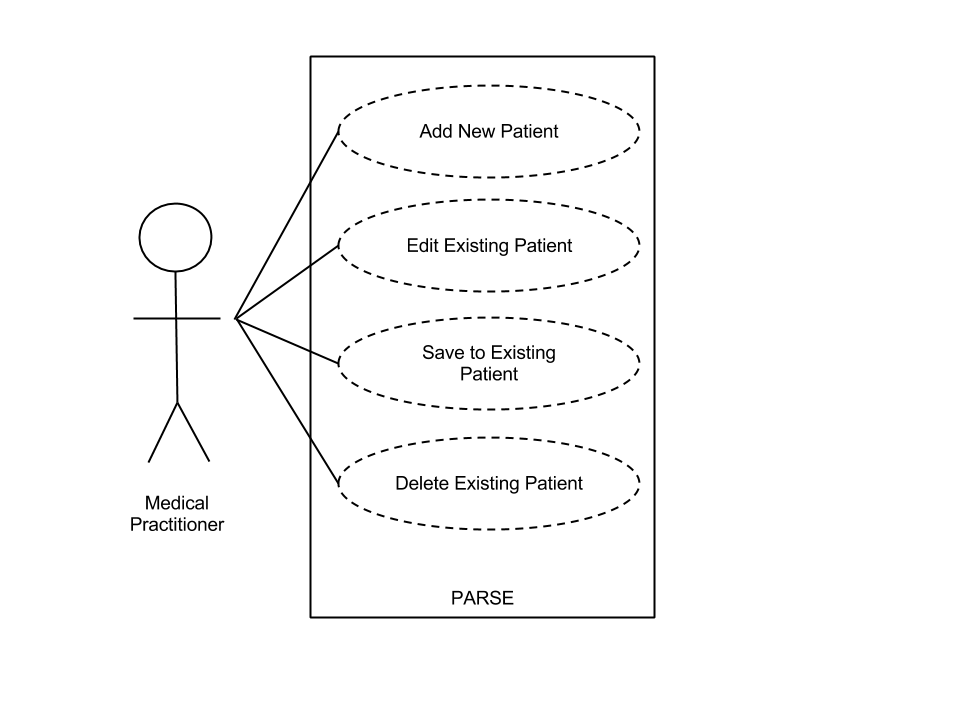
\includegraphics[scale=0.275]{images/uml5.png}
\end{center}

\subsection{Storage Requirements}

Each patient that is scanned into the system has their details recorded as part of the basic patient information system functionality that the toolkit provides. This patient information is required so that repeated volume or limb circumference scans or the markerless tracking of a medical measurement device can be attributed to the patient so that these measures can be monitored. The system uses a compact SQL relational database to store patient information and scan data. The inclusion of a database is important to the overall coherent functionality of each of the separate functions; the design of which is discussed below. \\

\subsection{Database}
For the storage requirements of the toolkit, a database has been put in place and it is used to store the details of the patients and their scans and measurements. To assist in the storage and retrieval of information from the database a specific class has been designed, that includes all the required queries. All accesses to the database are done in a clean and efficient way by using parameterised queries (otherwise called prepared statements). This not only enables re-usability of queries for different tables and sets of data but also makes the usage of the database safer as they provide protection against SQL injection attacks. \\

The toolkit also stores point cloud data in a proprietary \texttt{.PARSE} file format. These files are a serialized representation of the scans that are produced by the toolkit and are approximately 20mb in size for each point cloud produced. These are stored in the installation directory of the toolkit and their file directory reference stored in the database for later retrieval. The storage and retrieval of these point cloud files is achieved in \emph{O(n)} time.

\newpage

\subsection{Overall System}

As described in Section 3.1.1, the system's functionality has been designed so that each function is facilitated by a central class that encapsulates the functionality of the Kinect such that its streams can only be accessed by a single class at a time preventing multiple access instances from being possible and therefore preventing any unsafe states from being possible during normal operation of the system. \\

\subsection{Language Selection}

During the research and prototyping stages of the toolkit, a number of programming languages and libraries were investigated for their potential inclusion in the toolkit. C++ has particularly strong support for applications to Image Processing with the OpenCV\footnote{OpenCV, \emph{http://opencv.org/}} image processing library amongst others. These included algorithms such as SIFT and Haar that could potentially be used for identifying an object in a relatively sparse feature space. C++ also benefited from the (Point Cloud Library)\footnote{PCL, \emph{http://pointclouds.org/}} which included algorithms for point cloud reconstruction and cloud registration. The majority of related work had used elements of these libraries and had leveraged the use of C++ in their projects. However, prototyping using a C++ environment highlighted issues with including these frameworks into a collaborative development environment, the lack of a clear user interface framework and the learning curve associated with C++ required on behalf of all group members. \\

It was decided that C\# was a more suitable option due to its familiar programming constructs when compared to other mainstream object oriented languages and i's stability when it came to team development. The lack of library support has meant that development of particular aspects of the project has often not relied on these libraries or frameworks but has arguably led to a greater understanding and appreciation of these image processing and point cloud concepts by the group. It is also worth noting that there is no established work currently which uses the .NET framework for point cloud processing in the way we have done.

\subsection{Scope and Limitations}

The scope of the system is in line with the functional and non-functional requirements defined in the specification. Limitations imposed on the project have been due to the technical choices made in the design of the toolkit and also what has been necessary to fulfil the success criteria that was defined at the start of the project. \\

The system should be capable of producing reasonably accurate volume measurements and limb circumferences from a point cloud representation that can be saved and recalled. Such metrics should be atomic and measurable so that changes in limb circumference and body volume can be monitored over time. The visualisation of these scans should be representative of the quality of the scan. The system should also be capable of accurately recording and recalling the positioning of a scanner for medical measurement purposes and highlight areas where this is to occur appropriately. \\

Given the evolving nature of the technology, the team encountered several technical challenges and changes to the API provided by the Kinect as recent as March 2013 \cite{SDK13}. Including any changes from the API that supersede the design of the project was deemed out of scope so that sufficient testing time could be allowed for the existing framework. Apart from specific metrics concerning limbs and volume, the added recording of other body composition was also considered out of scope. The capturing of this data would have required additional hardware and the approximations of this data possible through the data captured by the Kinect (such as the calculation of the Siri body fat percentage based on body densities and height) has allowed this functionality to be retained without performing out of scope activities. \\

The nature of the scanning configuration was also important to consider in the design and by determining the optimal manner in which to capture the human body using the Kinect, we were able to reduce the amount of time spent prototyping different solutions. Patients are scanned four times in a static sensor configuration. This novel aspect of our project reduced the amount of time and complexity in setting up and performing the scan compared to other solutions which have either relied on multiple scanners \cite{Zhou2012} or a time of flight configuration resulting in a more computationally expensive volume reconstruction process. While this may yield a more accurate capture, the difference in precision has been considered minimal enough to use a four scan configuration. \\

The limitations of the design are highlighted by the out of scope activities above but such limitations could be acted upon in the future. \\

\section{Feasibility}

This project has a significant research and prototyping component due to the novel combination of functionalities that have been proposed. Given our extensive research into the capabilities of the Kinect and related work, we have deemed this project to be feasible in so far that we will be able to deliver the minimum functionality as specified in the project specification. It is safe to assume that further feasibility studies would have to be carried out once more extensive testing of the system has been carried out and for the system to be considered practical for initial diagnostic purposes in a realistic medical environment.

\section{Quality Assurance}

\begin{center}
    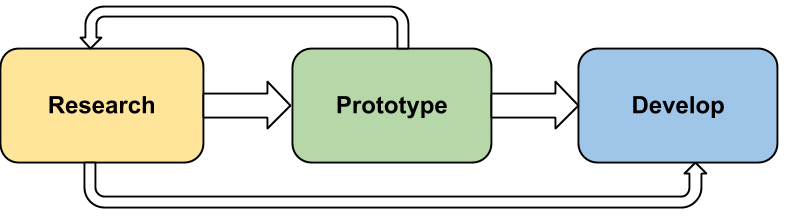
\includegraphics[scale=0.3]{images/developmentparse.png}
\end{center}

The quality of the system is assessed by considering the principles of Software quality assurance \cite{Chemuturi2010}. At each stage of the project we have adopted the approach  of researching, prototyping and then developing from these stages if appropriate. This has allowed us to measure each of our research and development goals against one another and against the requirements specified at the start of project. This means that we are able to assure quality of the deliverables in terms of how it compares to the research which has informed it and how well it meets the predetermined requirements.



